\chapter{Progettazione}
All'interno di questo capitolo andremo a discutere dei vari progetti svolti nella fase di tirocinio presso Ericsson Telecommunication con sede a Pagani per un periodo che intercorre tra Maggio a Dicembre del 2019 andandoci a soffermare sui contributi individuali. Ericsson Telecommunication ha istanziato dei fondi per poter produrre progetti sperimentali basati su nuove tecnologie in campo ICT e, nello specifico, nell'utilizzo delle reti che verranno adattate alla generazione 5G. Questo capitolo si baserà sulla progettazione dei vari casi d'uso dei prototipi applicativi basati sulla gestione di una rete secondo il modello basato su blockchain e, nello specifico, con l'utilizzo dell'infrastruttura permissioned fornita da Hyperledger Fabric. L'implementazione inerente a tali progetti verrà discussa nel capitolo successivo. I vari casi sviluppati hanno varie caratteristiche comuni che non hanno subito modifiche in fase implementativa dovuti alla flessibilità di Hyperledger Fabric e la sua adattabilità in vari contesti differenti. Ci siamo occupati di due casi d'uso principali:
\begin{enumerate}
    \item Healthcare: Basato su applicazioni in grado di poter gestire dati sanitari propri di un paziente in un contesto sicuro in cui il cliente era in grado di manipolare i permessi di accesso ai suoi dati privati e sensibili in maniera diretta e senza l'ausilio di terze parti. Nello specifico, si è visto come l'architettura abbia un ottimo utilizzo per le proposte di terapie in risposta ad analisi patologiche registrate dentro il sistema da ospedali. Poichè tali dati sono propri di ogni paziente, egli è l'unico in grado di poter rendere visibile tali informazioni a società terze come cliniche private e centri medici che sono le possibili fornitrici di terapie. Nel caso si dia il consenso alla visualizzazione di tali dati, qualsiasi società terza inclusa nel sistema non potrà ricondurre le informazioni che riceve con la persona reale dato che tali dati verranno rappresentati in forma anonima. 
    \item Automotive: Basato su applicazioni in grado di poter simulare la raccolta dati di sensori montati su componenti automobilistiche in cui la visualizzazione dei dati raccolti è gestita in maniera anonima all'interno di dashboard specifiche per componente, accessibili da società di fornitura esterne autorizzate o aziende proprietarie del prodotto. Il caso d'uso verifica anche come Hyperledger Fabric risponde al sovraccarico di lavoro provocato da continui inserimenti e accessi in rete che sviluppano transazioni da annettere in vari blocchi e leggono le informazioni legate allo stato globale del ledger.
\end{enumerate}
\section{Architettura di base}
L'architettura alla base dei vari progetti sviluppati si basa su una struttura in cui si contraddistinguono varie componenti in comunicazione. Ogni componente fornisce o richiede un servizio internamente all'architettura. Ci soffermeremo particolarmente su come le varie componenti si comportano in ambito di sicurezza andandone a definire i livelli per ogni strato dell'architettura.
\begin{figure}[h]
    \centering
    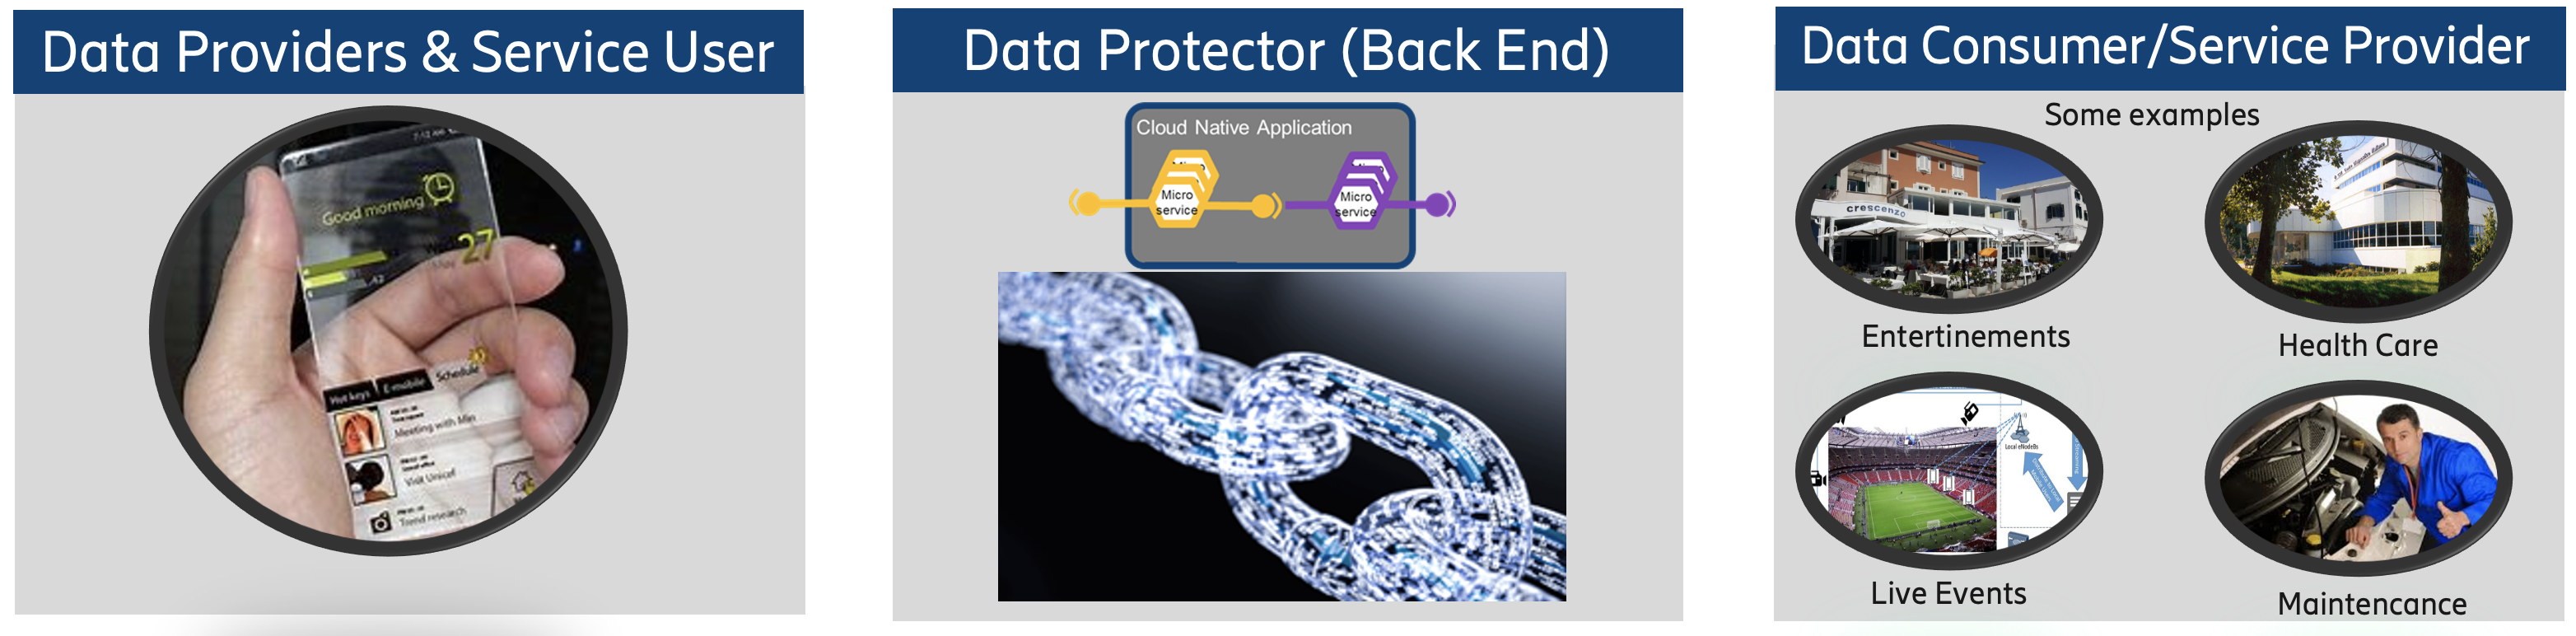
\includegraphics[width=1\textwidth]{img/structure-project-ericsson.png}
    \caption{Gestione della privatizzazione dei dati secondo l'architettura vista ad alto livello}
    \label{fig:architecture-private-diagram}
\end{figure}
\subsection{Progettazione degli strati }
L'architettura del prototipo si basa su una comunicazione che parte da un client (data producer o service provider) rappresentato da un'applicazione mobile o da una interfaccia web in grado di poter richiedereo visualizzare in maniera trasparente i dati con cui si interagisce. Il client comunica direttamente con un server REST appropriato a secondo del tipo di collezione e di operazioni che si intendono manipolare. Ogni server REST avrà, all'interno delle sue funzionalità, tutti i servizi che sono permessi a una specifica organizzazione di peer della blockchain sottostante implementata secondo la struttura logica offerta da Hyperledger Fabric. Il server dispone, quindi, di una serie d'invocazioni a funzioni abilitate per una specifica organizzazione andando a propagare i dati della richiesta del client e inoltrando la risposta fornita dai peer dell'organizzazione che rappresenta. Di seguito andremo a sintetizzare le caratteristiche principali di ogni componente in modo da rappresentare una panoramica generale sul flusso di esecuzione delle attività proposte all'interno del progetto.
\paragraph{Data Consumer e Service Provider}
Ogni client ha delle funzionalità in comune, tali funzioni interessano la gestione delle operazioni di base sulla blockchain della piattaforma che si vuole implementare, esse sono: 
\begin{enumerate}
    \item Registrazione di un nuovo account logico secondo una struttura basata sulla collezione del canale configurato della infrastruttura Fabric sottostante e mantenuta all'interno del ledger andandone a distinguere i vari attori a secondo di una visione fondata sul dominio delle funzionalità della business logic permesse. 
    \item Accesso ai dati dello stato globale del ledger secondo una visione specificata dai permessi di accesso dell'organizzazione. 
    \item Manipolazione dei dati dello stato globale del ledger a secondo dei permessi di visibilità e di accesso dell'organizzazione.
\end{enumerate}
Ciò che distingue i vari client non è solo la visione ad alto livello delle funzioni di cui dispone, ma anche come tali funzionalità sono gestite e visualizzate basandosi su criteri legati alla privatizzazione dei dati.
\paragraph{Server}
I server REST, invece, rispecchiano i servizi invocabili all'interno del chaincode installato all'interno dei canali collegati con i peer dell'organizzazione di riferimento. Lo scopo principale della scelta dell'uso di server di tipo REST è basata sulle proprietà di scalabilità proprie di ogni componente con gestione delle richieste in maniera asincrona. I server rappresentano un ponte che intercorre tra il client e la permissioned blockchain sottostante andando a definire una interfaccia pubblica utilizzabile legata alle invocazioni di funzioni del chaincode del canale Fabric di riferimento.  
\paragraph{Blockchain}
La blockchain rappresenta il contesto persistente di tutta l'architettura, adottandone un nuovo approccio basato sulla decentralizzazione dei dati su uno stato globale di un ledger distribuito e di operazioni di manipolazione o di accesso delle informazioni che generano transazioni mantenute all'interno di blocchi immutabili creati e validati da peer di rete e aggiunti all'interno della catena rappresentata dalla blockchain. 
Sotto un punto di vista logico, la blockchain fornisce contemporaneamente delle invocazioni a funzioni di manipolazione e persistenza dei dati basate su una struttura mantenuta all'interno di un chaincode istanziato dentro ogni peer collegato a un canale della rete e proprio di un canale logico di Hyperledger Fabric. I meccanismi di sicurezza si basano sul sistema di autenticazione basata sulle Certification Authorities e dei Membership Service Provider propri di Hyperledger Fabric cosi da evitare da semplificare il lavoro del programmatore che limita la gestione di questo aspetto solamente sulle possibili configurazioni delle componenti di sicurezza interne alla blockchain. 
\newpage
\section{Applicazione dell'adattabilità dell'architettura }
In seguito ad aver dato una spiegazione generale sulla struttura dell'architettura e su quali casi d'uso si voglia utilizzare, definiamo ora come si è svolto il lavoro progettuale sui due esempi implementati andando a soffermarci sui vari ostacoli che si sono affrontati.
\subsection{Caso d'uso: Healthcare}
La struttura della blockchain inerente a questo caso d'uso si basa sulla gestione di un singolo canale e di due organizzazioni. La prima organizzazione ha i peer che controllato il flusso logico inerente ai pazienti che interagiscono con la base di dati e gli ospedali, la seconda organizzazione, invece, fa riferimento a tutte le cliniche o società sanitarie esterne. Le due organizzazioni si distinguono per l'accessibilità alle collezioni interne al chaincode. Mentre i peer della prima organizzazione possono accedere ai dati pubblici e sensibili, la seconda organizzazione ha i diritti solo per la visibilità delle informazioni pubbliche. 
L'utilizzo di queste due organizzazioni è basata sui collegamenti verso due canali: Un pubblico e l'altro privato. Ogni organizzazione ha un server che definiscono le REST API utilizzabili da applicazioni esterne. Durante la fase di progettazione ad alto livello si sono distinti vari attori, ogni attore rientra in un dominio di permessi che, a sua volta, definisce il dominio delle applicazioni che interagiscono con ciascuna organizzazione. Di seguito riporteremo un'immagine riassuntiva dei ruoli principali che si sono prestabiliti in fase di progettazione: 
\begin{figure}[h]
    \centering
    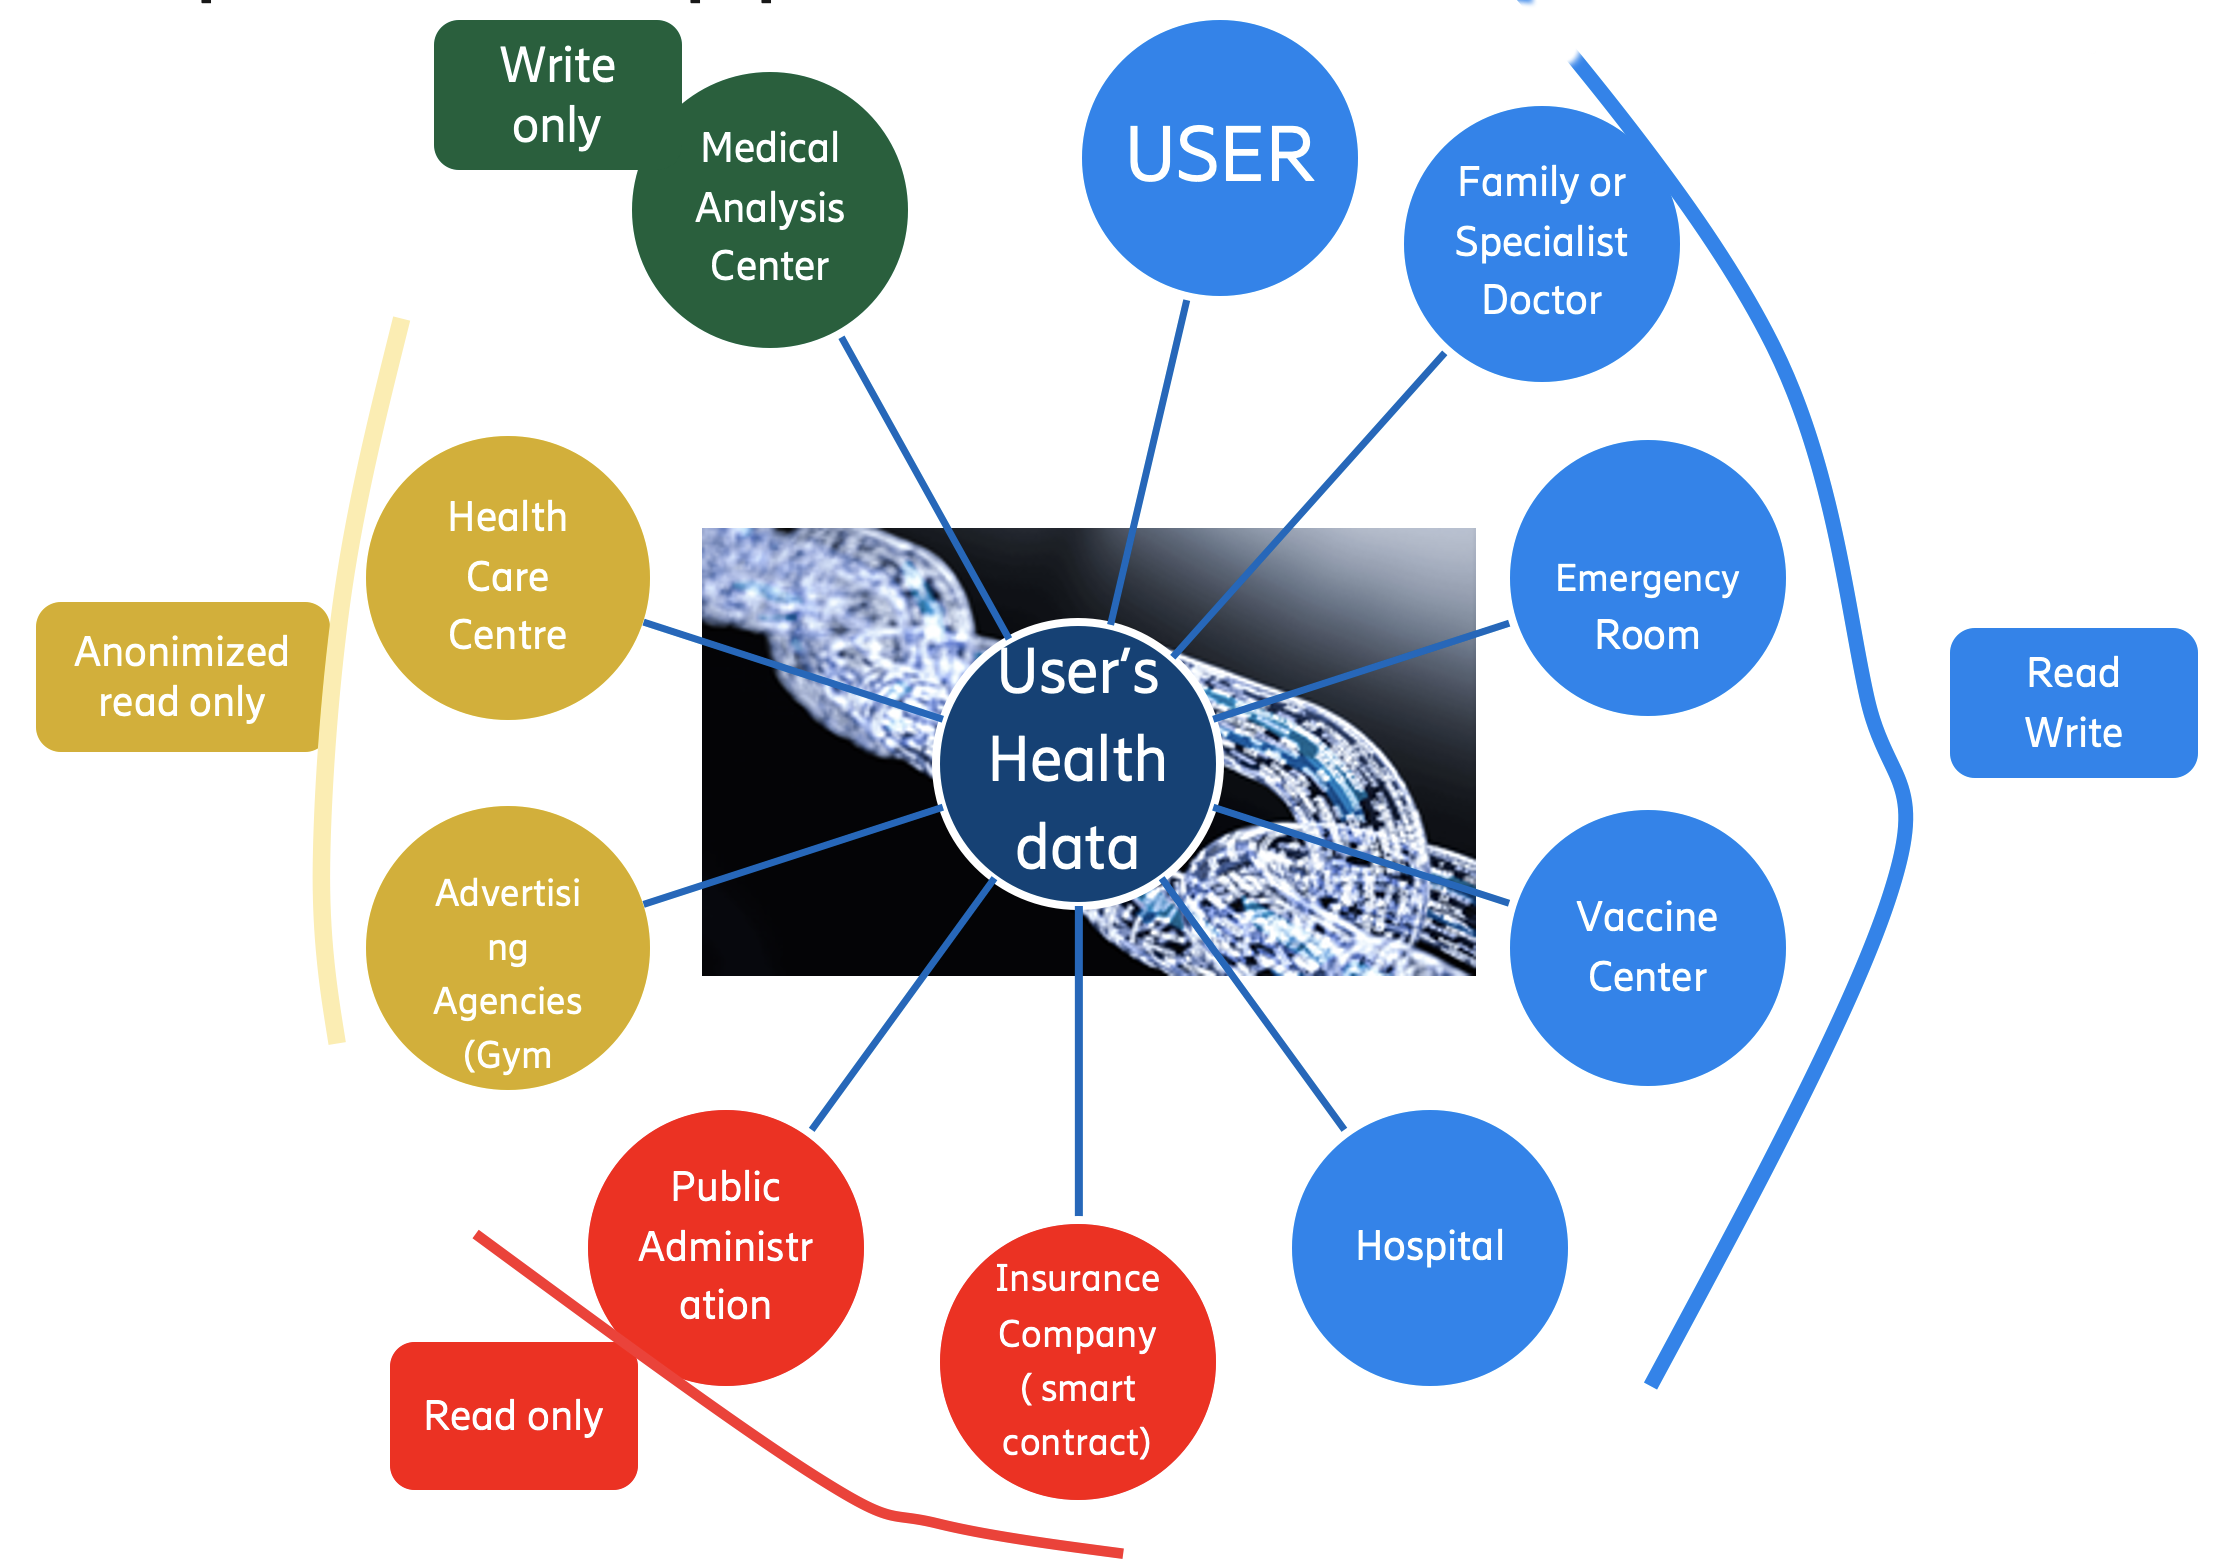
\includegraphics[width=0.6\textwidth]{img/actors-healthcare.png}
    \caption{Dominio progettuale degli attori per un ecosistema sanitario}
    \label{fig:actors-healthcare}
\end{figure}
All'interno della progettazione del prototipo, abbiamo concentrato la progettazione sulla manipolazione dei dati da parte di soli 3 tipi di attori, una per ogni categoria principale:
\begin{enumerate}
    \item User: Il paziente interessato alla gestione dei suoi dati pubblici, privati e sensibile. Ha la massima visibilità sui soli dati personali visualizzabili attraverso l'accesso a un applicazione mobile dedicata in cui poter vedere quali sono le informazioni gestite, andandone a manipolare i permessi e inserirne di nuove. I diritti apportati sono quelli definiti secondo i chaincode dei canali a cui fanno parte i peer della prima organizzazione.
    \item Ospedale: L'ospedale è un attore legato alla lettura e alla scrittura dei dati di ogni paziente ricevuto. Nello specifico, si occupa di leggere informazioni come intolleranze e allergie (dati sensibili) legati a un paziente e scrivere una qualsiasi patologia all'interno della sua cartella clinica decentralizzata e mantenuta dentro il ledger della blockchain. Non vi è nessun meccanismo di anonimizzazione dato che tale entità è autorizzata alla visualizzazione di qualsiasi forma d'informazione legate a una determinata persona sottoposta al processo sanitario. Come per l'utente, ha i permessi di lettura e di scrittura, andando ad accedere alle REST API e ai peer legate alla prima organizzazione.
    \item Centro medico: Il centro medico si occupa di ricevere delle patologie scritte all'interno delle cartelle cliniche di un paziente che ha accettato la condivisione dei suoi dati clinici da parte di società sanitarie esterne. Di seguito alla visualizzazione di queste patologie, è possibile scrivere una cura che verrà visualizzata dal paziente. Tutte le operazioni di scrittura e di lettura su dati visibili al centro medico sono anonimizzati, ciò significa che non sono accessibili i dati inerenti a informazioni personali che possono condurre i dati all'associazione con una persona reale. Tale attore interagisce con il ledger tramite i peer dell'organizzazione due, ciò fa si che accede solamente al canale pubblico senza avere nessuna autorizzazione per il canale privato.
\end{enumerate}
\subsubsection{Contributi individuali}
I contributi individuali sia in fase progettuale che in fase implementativa interessano l'implementazione del centro medico, delle REST API della seconda organizzazione con cui interagiscono i possibili service provider rappresentate da società esterne al sistema sanitario nazionale e dell'adattabilità della blockchain alla struttura desiderata andando a raffinare meccanismi come la configurazione delle policy per la visibilità, dell'accesso e della manipolazione del ledger.
\subsection{Caso d'uso: Automotive}
Altra parantesi si ha con il caso d'uso basato sul contesto dell'Automotive. All'interno della sua progettazione si ha come obiettivo principale quello di definire un sistema di monitoraggio per le componenti di un autovettura proprietaria in cui solamente chi ha i diritti di accesso verso il bene o una sua componente possono seguire in tempo reale le statistiche generate. L'adattabilità dell'architettura si basa sulla gestione di quattro organizzazioni all'interno della blockchain, ognuna legata ad aziende responsabili della fornitura o del possesso del bene. All'interno del prototipo abbiamo distinto tali componenti in freni, gomme, motore per i fornitori andando a lasciare un'organizzazione per l'azienda proprietaria o il proprietario dell'autovettura. Ogni componente è diviso in una collezione privata specifica, ogni organizzazione ha i diritti di visibilità sulla propria componente o, in caso si ci riferisce all'organizzazione proprietaria, su tutte le collezioni. Cosi facendo, i fornitori possono controllare problemi di prestazione su una particolare auto in movimento senza interessarsi delle altre componenti.
La struttura dell'architettura adattata per tale caso d'uso si presenta secondo tali principali componenti:
\paragraph{Client} 
All'interno della progettazione del prototipo, i client di riferimento si dividono in due tipi: 
\begin{itemize}
    \item Client di simulazione: In cui hanno la funzione di aggiornare i dati all'interno dello stato globale del ledger.
    \item Client di visualizzazione: In cui hanno la funzione di leggere i dati dei valori di alcune collezioni contenute all'interno dello stato globale del ledger. 
\end{itemize}
Il client simulatore progettato ha il compito d'inserire, con frequenza costante, dei dati che simulano il comportamento delle componenti su un auto in movimento. Tali aggiornamenti andranno a creare dei blocchi all'interno della blockchain in cui le transazioni conterranno lo stato dei parametri delle componenti in un determinato istante durante la fase di movimento di un auto. I client di visualizzazione che si sono progettati, invece, hanno il compito di leggere lo stato globale nelle sole collezioni in cui hanno autorizzazioni. Tali client si presenteranno come delle dashboard che andranno a visualizzare e confrontare i dati ricevuti graficamente.
\paragraph{Server}
I server sviluppati seguono la stessa logica del caso d'uso Healthcare, in questo caso avremmo quattro server REST che forniscono un'interfaccia pubblica per l'invocazione di funzioni autorizzate all'organizzazione di riferimento.
\paragraph{Blockchain}
La blockchian sottostante distingue i permessi per quattro Membership Service Provider legate alle quattro organizzazioni che elaborano su un medesimo ledger distinguendone la visione secondo i soli permessi andandone a distinguere un canale privato da uno pubblico logico e differente per i peer delle varie organizzazioni.
\subsubsection{Contributi individuali}
All'interno della progettazione del caso d'uso e dell'implementazione del prototipo, ho sviluppato le dashboard, andando ad adattare i server REST all'interfaccia pubblica da e verso le collezioni della blockchain. Inoltre, sono stato il responsabile dell'architettura interna della blockchain andando a definire e configurare i vari peer delle varie organizzazioni andando ad adattare la definizione e l'istanziazione dei chaincode, del ledger e della logica di business del canale tramite le policy di configurazione di Fabric.
\section{Osservazioni finali in fase di progettazione}
All'interno delle conclusioni della fase di progettazione dei protitipi, si vuole fornire un differente fine all'interno dei due casi d'uso. Mentre all'interno del contesto sanitario vogliamo filtrare i dati, andando ad anonimizzare le identità dei pazienti a secondo della tipologia di attore che interagisca con la blockchain, all'interno del secondo caso d'uso, abbiamo anonimizzato i dati a secondo del tipo di attore ma si ha avuto maggior interesse nel vedere come Hyperledger Fabric rispondeva al sovraccarico di lavoro definendo cosi anche i limiti dell'architettura.
\newpage 